\documentclass[a4paper,12pt]{article} % Document class

% Packages
\usepackage[utf8]{inputenc} % Encoding
\usepackage{amsmath} % For mathematical formulas
\usepackage{graphicx} % For including images
\usepackage{hyperref} % For hyperlinks
\usepackage{titling} % For custom title
\usepackage{pdflscape} % For landscape pages
\usepackage{tabularx} % For flexible column widths
\usepackage[margin=2.5cm]{geometry} % Adjust the margin here (e.g., 2.5cm)
\usepackage{graphicx} % For including images
\usepackage{multirow}
\usepackage{listings} % import and format code from an external file



% Set default path for images
\graphicspath{{../img/}}

% Prevent hyphenation globally
\hyphenpenalty=10000
\exhyphenpenalty=10000

\title{Web Technologies \\
        \large{Exercise Sheet 2 -- Web-Shop - CSS}} % Title
\author{Team 3: Jiahui~Dai, Yana~Halamakh, Wei~Wei~Tang} % Author
\date{\today} % Date

\begin{document}

\maketitle % Create title
\hrule % Create a horizontal line
\tableofcontents % Create table of contents
\newpage

\section{Registeration, Login, Customer Profile}

\subsection{\texttt{form-validation.js}}
\lstinputlisting{../../src/script/form-validation.js} 

\section{Conceptual Model}
Please refer to  Figure~\ref{fig:task2} for the structural workflow model of our website.
% To redraw diagram.

\begin{figure}[h]
    \centering
    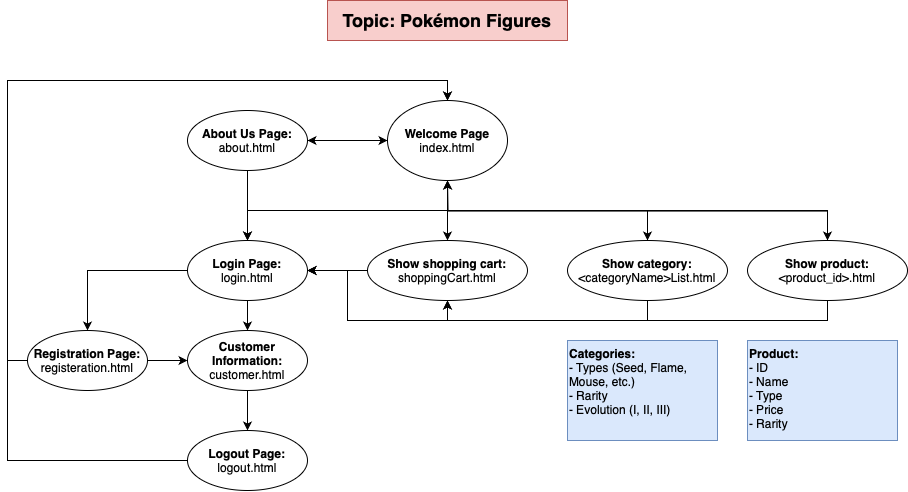
\includegraphics[width=\textwidth]{conceptual-model.drawio.png} % Adjust the path and file name
    \caption{Conceptual Model for Web-Shop}
    \label{fig:task2}
\end{figure}
\section{\texttt{index.html}}

\lstinputlisting[language=HTML]{../../src/index.html}






% END OF DOCUMENT
\begin{center}
    \vspace{5em}
    \textbf{END OF DOCUMENT}
\end{center}


\end{document}
